\section{Airborne vs.\ Mechanical Coupling}\label{sec:coupling}

Having established that the abdomen possesses flexural resonances squarely
in the infrasonic range, we now ask whether airborne sound can
actually \emph{excite} them.  Under realistic airborne
exposure conditions, the answer is effectively no.

\subsection{Airborne Acoustic Pathway}

At \SI{4}{\hertz}, the acoustic wavelength in air exceeds \SI{85}{\metre}---
some 500 times the abdominal radius.  In this regime the abdomen is
acoustically compact.  Table~\ref{tab:airborne} quantifies the resulting weak
coupling.  The energy-consistent displacement in column~3 is derived from the
absorption cross-section (Eq.~\ref{eq:sigma_abs} below); the reciprocity
argument is developed fully in \S\ref{sec:energy_budget}.  Modern analyses of
scattering by pressurised elastic shells reach the same qualitative
conclusion: long-wavelength radiation and absorption by low-order shell modes
are strongly suppressed \cite{Godin2023}.

\begin{table}[htbp]
  \centering
  \caption{Energy-consistent airborne displacement at $n=2$ resonance
  ($f_2 = \SI{4.0}{\hertz}$, $Q = 4.0$, canonical parameters).
  Displacements scale linearly with incident pressure; intermediate values may
  be interpolated.  The pressure-based upper-bound estimate overestimates by a
  factor of ${\approx}\,6.5$ (ratio of $\xi_\mathrm{pressure}$ to
  $\xi_\mathrm{energy}$).}
  \label{tab:airborne}
  \begin{tabular}{rcccc}
    \toprule
    SPL (dB) & $p_\mathrm{inc}$ (Pa) &
    $\xi_\mathrm{energy}$ ($\mu$m) &
    $\xi_\mathrm{pressure}$ upper bound ($\mu$m) & Energy-consistent $>\SI{1}{\micro\metre}$? \\
    \midrule
    120 & 20.0 & 0.028 & 0.18  & No \\
    151 & 710  & 0.99  & 6.4   & Nearly \\
    \bottomrule
  \end{tabular}
\end{table}

At the $n = 2$ resonance, the energy-consistent airborne transfer function is
\begin{equation}
  H_\mathrm{air}(\omega_2)
  = \frac{\xi}{p_\mathrm{inc}}
  \approx 1.4 \times 10^{-9}\,\si{\metre\per\pascal}.
  \label{eq:H_air}
\end{equation}
The displacements in Table~\ref{tab:airborne} therefore scale linearly with
incident pressure.

At \SI{120}{\decibel} SPL---a level exceeding the conventional threshold of
discomfort, and roughly the level at
which conversation becomes impossible---the energy-consistent wall
displacement is \SI{0.028}{\micro\metre}.  This falls two orders of magnitude
below the $0.5$--$\SI{2.0}{\micro\metre}$ cellular activation range of
mechanosensitive PIEZO1 and PIEZO2 channels \cite{coste2010piezo1}, a
benchmark derived from cell-culture experiments that provides a useful
order-of-magnitude reference scale for biological mechanosensitivity.
Reaching the
\SI{1}{\micro\metre} cellular benchmark on this energy-consistent basis demands
approximately \SI{151}{\decibel} (cf.\ \SI{135}{\decibel} using the
pressure-based upper-bound displacement, which overestimates by
${\approx}\,6.5\times$), a level associated with severe
acoustic hazards and available only from explosive blasts and rocket launches.
Modern mechanobiology strengthens rather than weakens that conclusion:
PIEZO1 gating is tuned by membrane tension in the low-\si{\milli\newton\per\metre}
range, with half-maximal activation near \SI{2}{\milli\newton\per\metre}
\cite{Lewis2015}.  While the membrane-tension thresholds reported in
cell-culture experiments cannot be directly translated to tissue-scale
displacements, the order-of-magnitude comparison remains informative.  Recent
reviews summarise the broader physiological roles of PIEZO channels
(following the 2021 Nobel Prize, and with structural detail from cryo-EM
\cite{Saotome2018}) \cite{Xiao2024}.  Of particular relevance here,
PIEZO2-dependent
gut mechanosensation is now known to regulate gastrointestinal transit
\cite{ServinVences2023}.  The relevant question is therefore not whether the
gut can sense deformation---it plainly can---but whether airborne infrasound
can generate enough deformation.  At such levels, auditory injury would be the
more immediate clinical hazard than gastrointestinal effects.

\subsection{Mechanical (Whole-Body Vibration) Pathway}

Mechanical vibration, by contrast, bypasses the acoustic
impedance barrier entirely.  Vibration transmitted through the
skeleton couples directly to the abdominal wall, bypassing the $(ka)^n$
penalty entirely.  Because the bone--peritoneum impedance contrast is orders
of magnitude smaller than the air--tissue mismatch, an upper-bound
base-excitation model that assumes rigid skeletal transmission
captures the essential physics \cite{FahyGardonio2007,Gupta2021}.
Table~\ref{tab:mechanical} shows substantially stronger coupling.

\begin{table}[htbp]
  \centering
  \caption{Mechanical coupling at $n=2$ resonance
  ($f_2 = \SI{4.0}{\hertz}$, $Q = 4.0$, $\Gamma_2 = 1$).  The EU Directive 2002/44/EC
  action value is \SI{0.5}{\metre\per\second\squared}.  Displacements scale
  linearly with base acceleration; intermediate values may be interpolated.
  The corrected values (\S\ref{sec:coupling_ratio}) use $\Gamma_2 = 0.48$.}
  \label{tab:mechanical}
  \begin{tabular}{rcccc}
    \toprule
    $a_\mathrm{rms}$ (m/s$^2$) & $x_\mathrm{base}$ ($\mu$m) &
    $\xi_\mathrm{rel}$ ($\mu$m) &
    $\xi_\mathrm{corr}$ ($\mu$m)\textsuperscript{$\dagger$} &
    Exceeds 1\,\si{\micro\metre}? \\
    \midrule
    0.1 & 229  & 917  & 440  & Yes \\
    0.5 (EU action) & 1147  & 4586 & 2201 & Yes \\
    \bottomrule
    \multicolumn{5}{l}{\textsuperscript{$\dagger$}Corrected for
      modal participation: $\xi_\mathrm{corr} = \Gamma_2\,\xi_\mathrm{rel}$
      with $\Gamma_2 = 0.48$.}
  \end{tabular}
\end{table}

At the same resonance, the corresponding SDOF mechanical transfer function is
\begin{equation}
  H_\mathrm{mech}(\omega_2)
  = \frac{\xi}{a_\mathrm{rms}}
  \approx 9.17 \times 10^{-3}\,\mathrm{m}/(\mathrm{m\,s^{-2}}).
  \label{eq:H_mech}
\end{equation}
before the modal-participation correction discussed below.

At the EU action value of \SI{0.5}{\metre\per\second\squared}, the predicted
displacement exceeds the PIEZO cellular benchmark by more than three orders of
magnitude.  Unlike the airborne case, this is not a theoretical curiosity:
it is consistent with occupational exposures among operators of heavy
equipment, long-haul drivers, and helicopter pilots, in whom gastrointestinal
complaints are well documented
\cite{Griffin1990}.  Recent seated-body biodynamic studies likewise
show strong low-frequency nonlinearity, cross-axis coupling, and identifiable
abdominally relevant modes in this same band \cite{Zheng2012,Gao2021}.

\subsection{The Coupling Ratio}
\label{sec:coupling_ratio}

The system property of interest is the pair of transfer functions in
Eqs.~\eqref{eq:H_air} and \eqref{eq:H_mech}, not a single universal
dimensionless number.  For any chosen airborne pressure and mechanical
acceleration, the corresponding displacement ratio is
\begin{equation}
  \mathcal{R}(\omega)
  = \frac{H_\mathrm{mech}(\omega)\,a_\mathrm{rms}}
         {H_\mathrm{air}(\omega)\,p_\mathrm{inc}}.
  \label{eq:coupling_ratio}
\end{equation}
Equation~\eqref{eq:coupling_ratio} is therefore pair-specific: the dimensionless
ratio depends on the selected exposure levels.  At the $n = 2$ resonance, the
transfer-function ratio itself,
\[
  \frac{H_\mathrm{mech}}{H_\mathrm{air}}
  \approx 6.5 \times 10^{6}\,\si{\pascal\second\squared\per\metre},
\]
is a property of the shell--fluid system.  Using
$p_\mathrm{inc} = \SI{20}{\pascal}$ (\SI{120}{\decibel} SPL) and
$a_\mathrm{rms} = \SI{0.1}{\metre\per\second\squared}$ gives the headline SDOF
upper bound
\[
  \mathcal{R}_\mathrm{full}
  \approx \frac{9.17 \times 10^{-3}\times 0.1}
                {1.4 \times 10^{-9}\times 20}
  \approx 3.3 \times 10^{4}.
\]
Equivalently, to produce the same abdominal-wall displacement as
\SI{120}{\decibel} SPL airborne exposure, the required mechanical acceleration
is only
\begin{equation}
  a_\mathrm{eq}
  = \frac{H_\mathrm{air}\,p_\mathrm{inc}}{H_\mathrm{mech}}
  \approx 3.1 \times 10^{-6}\,\si{\metre\per\second\squared},
  \label{eq:a_eq}
\end{equation}
which is 5.2 orders of magnitude below the EU occupational action value of
\SI{0.5}{\metre\per\second\squared}.  The precise dimensionless ratio changes
with the chosen reference pressure and acceleration, but the qualitative
ordering---mechanical coupling far exceeding airborne coupling---is independent
of that choice because it rests on the large transfer-function ratio
$H_\mathrm{mech}/H_\mathrm{air}$.  The ratio carries units of
\si{\pascal\second\squared\per\metre}; obtaining a dimensionless comparison at
any frequency requires choosing a reference pressure and acceleration, but the
enormous gap persists for all realistic exposure pairings.

\paragraph{Modal participation.}
Vertical base excitation displaces the constrained portion rigidly, imposing a
velocity boundary condition on the free shell at $\theta = \theta_c$.
Figure~\ref{fig:constraint_geometry} defines the corresponding geometry.  The
mechanical displacement in Eq.~\eqref{eq:coupling_ratio} assumes perfect
coupling of vertical base excitation into the $n=2$ mode (modal participation
factor $\Gamma_2 = 1$).  The participation factor for mode~$n$ under vertical
base excitation of the oblate spheroid is
\begin{equation}
  \Gamma_n
  = \frac{a\,\displaystyle\left|\int_{\cos\theta_c}^{1}
      \eta\,P_n(\eta)\,\mathrm{d}\eta\right|}
    {\displaystyle\int_{-1}^{1}
      P_n^{2}(\eta)\,\sigma(\eta)\,\mathrm{d}\eta},
  \label{eq:participation_factor}
\end{equation}
where $\eta = \cos\theta$, $P_n$ is the Legendre polynomial of degree~$n$,
$\theta_c$ is the polar angle below which the shell is rigidly constrained
by the pelvis and spine, and
$\sigma(\eta) = \sqrt{c^{2} + (a^{2}-c^{2})\,\eta^{2}}$
is the oblate-spheroid surface metric factor.  The numerator integral
quantifies the overlap between the vertical base-displacement pattern
($\propto \cos\theta = \eta$) and the mode shape $P_n(\eta)$ over the
unconstrained cap; the denominator normalises that overlap by the corresponding
modal mass on the full oblate surface.  In this convention, $\Gamma_n$ measures
how efficiently rigid vertical support motion projects onto the $n$th shell
mode.

\begin{figure}[htbp]
  \centering
  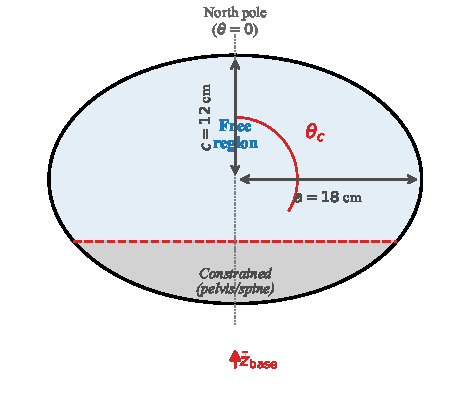
\includegraphics[width=0.58\textwidth]{figures/fig_constraint_geometry.pdf}
  \caption{Constraint geometry for vertical base excitation.  The inferior
  portion of the shell is rigidly supported below the polar angle $\theta_c$,
  representing pelvic and spinal attachment, while the superior cap remains
  free to deform.}
  \label{fig:constraint_geometry}
\end{figure}

For a free sphere ($\theta_c = \pi$), the numerator reduces to
$\int_{-1}^{1} \eta\,P_n(\eta)\,\mathrm{d}\eta$, which vanishes for $n \neq 1$
by Legendre orthogonality; a free sphere therefore has $\Gamma_2 = 0$ exactly.
At the opposite extreme, $\theta_c \rightarrow 0$ leaves no unconstrained cap,
so the overlap integral also vanishes.  Partial skeletal constraint breaks the
free-sphere orthogonality and yields finite coupling into the $n=2$ mode.

\begin{figure}[htbp]
  \centering
  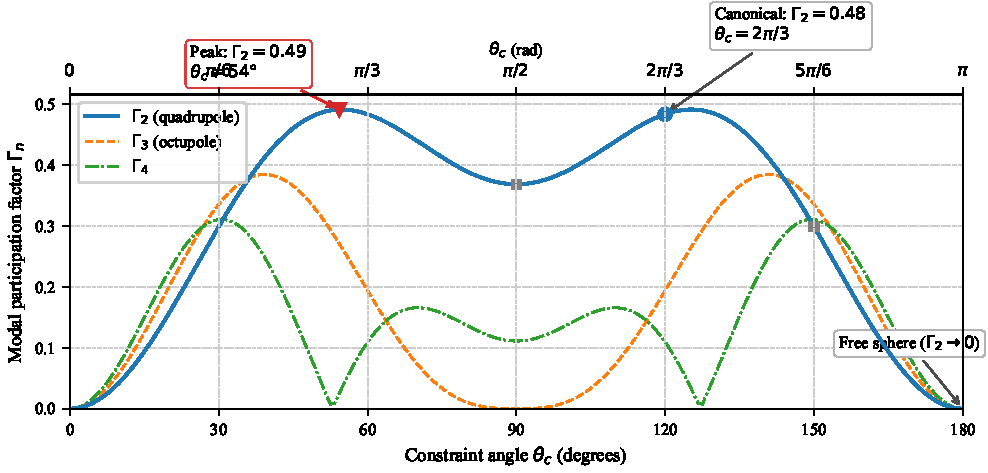
\includegraphics[width=0.72\textwidth]{figures/fig_gamma2_thetac.pdf}
  \caption{Modal participation factor $\Gamma_2$ as a function of constraint
  angle $\theta_c$ for the canonical oblate shell ($a = \SI{0.18}{\metre}$,
  $c = \SI{0.12}{\metre}$).  The factor vanishes at both extremes: fully
  clamped ($\theta_c = 0$) and free ($\theta_c = \pi$).  The canonical pelvic
  constraint ($\theta_c = 2\pi/3$, dashed line) gives $\Gamma_2 \approx 0.48$.}
  \label{fig:gamma2}
\end{figure}

The participation factor is non-monotonic in the constraint angle
(Fig.~\ref{fig:gamma2}): it vanishes at both extremes (fully clamped,
$\theta_c \rightarrow 0$, and free, $\theta_c = \pi$) and reaches a maximum
$\Gamma_2 \approx 0.49$ near $\theta_c \approx 125^\circ$.  At the canonical
pelvic constraint ($\theta_c = 2\pi/3$), $\Gamma_2 \approx 0.48$, close to the
peak; at $\theta_c = \pi/2$ (lower half constrained), $\Gamma_2 \approx 0.37$.
Including this correction reduces the mechanical displacement to about 48\% of
the SDOF value and the coupling ratio to $\sim 1.6 \times 10^4$.  The
qualitative conclusion---a four-order-of-magnitude gap---is unaffected, but
the uncorrected $\mathcal{R}_\mathrm{full}$ reported above should be understood
as an upper bound corresponding to the SDOF idealisation.

\subsection{Energy Budget}\label{sec:energy_budget}

We verify self-consistency through the absorption cross-section derived from
reciprocity \cite{Junger1986,Godin2023}.  The radiation efficiency of
low-order shell modes is vanishingly small when $ka \ll 1$
\cite{FahyGardonio2007}; formally:
\begin{equation}\label{eq:sigma_abs}
  \sigma_\mathrm{abs} = \frac{(2n+1)\lambda^2}{4\pi}
  \,\frac{4\,\zeta_\mathrm{rad}\,\zeta_\mathrm{struct}}{(\zeta_\mathrm{rad} + \zeta_\mathrm{struct})^2},
\end{equation}
where $\zeta_\mathrm{rad}$ and $\zeta_\mathrm{struct}$ are the radiation and
structural damping ratios, respectively.  For the $n=2$ mode in air,
$\zeta_\mathrm{rad} \approx 10^{-15}$ whereas
$\zeta_\mathrm{struct} = 0.125$, giving a Breit--Wigner absorption efficiency
$4\zeta_\mathrm{rad}\zeta_\mathrm{struct}/\zeta_\mathrm{total}^2
\sim 3 \times 10^{-14}$.  The shell absorbs roughly three parts in a hundred
trillion of the incident acoustic energy.

The energy-consistent displacement follows directly.  The absorbed acoustic
power is $\Pi_\mathrm{abs} = \sigma_\mathrm{abs} \, I$, where
$I = p_\mathrm{inc}^2 / (2 \rho_\mathrm{air} c_\mathrm{air})$ is the
free-field intensity.  At steady-state resonance, the time-averaged
dissipated power is
$\langle P_\mathrm{diss}\rangle = c_\mathrm{eq}\langle\dot{x}^2\rangle$,
where the equivalent viscous damping coefficient is
$c_\mathrm{eq} = 2\zeta\omega_n M_\mathrm{eff}$ and the mean-square
velocity of a harmonic oscillation with amplitude $\xi$ is
$\langle\dot{x}^2\rangle = \omega_n^2\xi^2/2$.  Hence
$\langle P_\mathrm{diss}\rangle = \zeta\omega_n^3 M_\mathrm{eff}\xi^2$.
Equating absorbed and dissipated power gives
\begin{equation}\label{eq:xi_energy}
  \xi_\mathrm{energy}
  = \sqrt{\frac{\sigma_\mathrm{abs}\,I}
               {\zeta_\mathrm{struct}\,\omega_n^3\,M_\mathrm{eff}}},
\end{equation}
where $M_\mathrm{eff} = m_\mathrm{eff}^{(n)} \times 4\pi R^2$ is the total
modal mass.  The $(2n+1)$ partial-wave degeneracy in $\sigma_\mathrm{max}$
and the corresponding $1/(2n+1)$ modal-mass normalisation cancel for the
single azimuthal order excited by a plane wave.
The factor of
$4\zeta_\mathrm{rad}\zeta_\mathrm{struct}/\zeta_\mathrm{total}^2
\sim 3 \times 10^{-14}$ inside $\sigma_\mathrm{abs}$ is the physical origin of the
${\approx}\,6.5\times$ reduction from the pressure-based upper bound
(equation~\ref{eq:xi_air}): the pressure-based calculation implicitly
assumes that all incident energy is available to drive the mode, whereas in
fact only the Breit--Wigner fraction
$4\zeta_\mathrm{rad}\zeta_\mathrm{struct}/\zeta_\mathrm{total}^2$ is absorbed.
The pressure-based upper bound (with unity prefactor) exceeds the
energy-consistent result by approximately $6.5\times$; with the exact
multipole coefficient of $1/3$ (\S\ref{sec:airborne}), the pressure-based
estimate reduces to approximately $0.06\,\mu\text{m}$, still a factor of
${\sim}\,2$ above the energy-consistent value.
This radiation inefficiency in the Rayleigh regime ($ka \ll 1$) is a
well-established result in structural acoustics \cite{Junger1986,FahyGardonio2007}.

\subsection{Comparison with Empirical Evidence}

The model predictions align with two otherwise contradictory bodies of
evidence:
\begin{itemize}
  \item \textbf{WBV studies}: ISO~2631 documents gastrointestinal symptoms
    at $4$--$\SI{8}{\hertz}$ under mechanical vibration \cite{iso2631}.
    Our model explains \emph{why} this frequency range is problematic.
  \item \textbf{Airborne infrasound studies}: No gastrointestinal effects
    have been observed at SPL $\leq \SI{150}{\decibel}$, although modern
    controlled exposure studies do report subtle neural effects without
    evidence of visceral resonance \cite{Leventhall2007,Ascone2021}.  Our
    model explains why gastrointestinal effects should not be expected.
\end{itemize}
The transfer-function disparity resolves this apparent contradiction
(Figure~\ref{fig:coupling}): both literatures concern the same abdominal
resonance, but through excitation pathways with markedly different coupling
efficiencies.

\begin{figure}[htbp]
  \centering
  
\includegraphics[width=\textwidth]{figures/fig_coupling_comparison.pdf}
  \caption{The central result.  Left: wall displacement vs.\ frequency for
  airborne excitation at \SI{120}{\decibel} SPL (lower curve) and mechanical
  whole-body vibration at \SI{0.5}{\metre\per\second\squared} (upper curve),
  showing a gap of roughly four orders of magnitude at resonance.
  Right: comparison of all four coupling pathways at the $n=2$ resonance;
  the horizontal dashed line marks the PIEZO cellular mechanosensory reference scale.}
  \label{fig:coupling}
\end{figure}
